% !TEX root = main.tex

\section{传输层} % transport layer
传输层协议称为\textemph{端到端}或\textemph{进程到进程}的协议。 因特网的传输层可以为两个进程在\textemph{不可靠的网络层}上建立一条\textemph{可靠的逻辑链路},提供\textemph{字节流}传输服务,并且可以进行\textemph{流控制}和\textemph{拥塞控制}。

因特网的传输层有两个协议:
\begin{itemize}
\item UDP协议提供\underline{无连接的不可靠尽力服务}(IP数据报协议字段\textemph{UDP为17})
\item TCP协议提供\underline{面向连接的可靠字节流服务}(IP数据报协议字段\textemph{TCP为6})
\end{itemize}

我们把传输层的数据单元(报文)称为\underline{数据段(segment)}。

每个TCP/UDP连接可以由一个四元组唯一标识:\underline{源IP地址、源端口号、目的IP地址、目的端口号},通过\textemph{端口号}区分不同进程。

而一对\underline{IP地址和端口号}就构成一个通信端点,也被称为\underline{套接字(socket)}。

\begin{itemize}
    \item 知名端口:0-1023,为提供知名网络服务的系统进程所用。如:
    \begin{center}
    \begin{tabular}{|c|c|c|c|}\hline
        80 & HTTP & 25 & SMTP\\\hline
        20 & FTP 数据 & 53 & DNS\\\hline
        21 & FTP 控制 & 110 & POP3\\\hline
        23 & Telnet & &\\\hline
    \end{tabular}
    \end{center}
    \item 注册端口:1024-49151。在IANA注册的专用端口号,为企业软件所用。
    \item 动态端口:49152-65535,没有规定用途的端口号,一般用户可以随意使用。也称为私用或暂用端口号。
\end{itemize}

\subsection{UDP协议}
\subsubsection{概述}
用户数据报协议(User Datagram Protocol, UDP)只提供\textemph{无连接的不可靠的尽力服务}。发送给接收进程的数据有可能\textemph{丢失},也有可能\textemph{错序}。
可以说UDP协议是IP协议的简单扩展,只是在IP协议上增加了\textemph{端口号},把进程关联起来了。
\begin{itemize}
\item UDP是\textemph{面向报文}的传输方式,即应用层交给UDP多长的报文,UDP就照样发送,每一次都发送一个报文。
既不合并,也不拆分,而是\textemph{保留}这些报文的\textemph{边界}。
\item 接收进程每次接收一个完整的数据报,如果进程设置的接收缓冲区不够大,收到的数据报将被截断。
\end{itemize}

\subsubsection{数据段格式}
\begin{figure}[H]
    \centering
    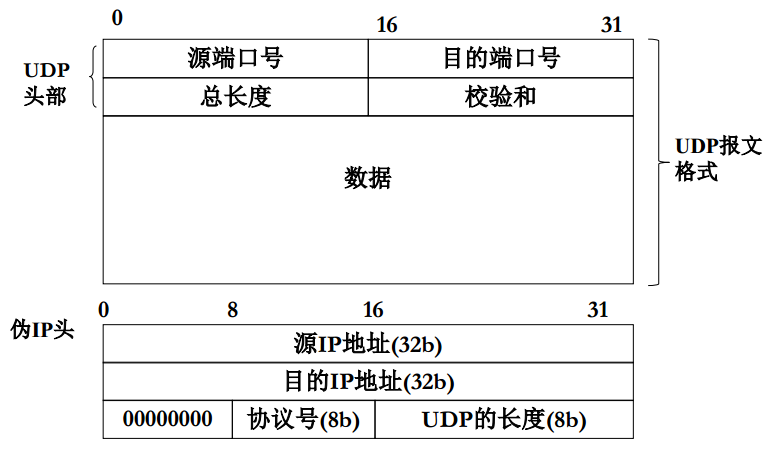
\includegraphics[width=0.6\linewidth]{fig/udp_format.png}
\end{figure}
\begin{itemize}
    \item 总长度:整个UDP报文长度
    \item 源端口号和目的端口号(2B):用于关联发送进程和接收进程
    \item 校验和:由\underline{伪IP头}(只用来算校验和,不进行传递)、\underline{UDP头}(校验和用0填充)和\underline{UDP数据}形成。
    其中,伪IP头的协议号为17。
    如果发送方把校验和设置为0,接收方会忽略校验和。
    UDP长度就是UDP头部填写的总长度。
\end{itemize}

\subsection{TCP协议}
\subsubsection{概述}
传输控制协议(Transmission Control Protocol, TCP)为进程之间提供\textemph{面向连接的可靠的}数据传送服务(通过滑动窗口协议实现)。TCP为\textemph{全双工}协议。TCP提供\textemph{流控制}机制,即控制发送方的发送速度,使发送的数据不会淹没接收方。作为因特网的主要数据发源地,TCP还提供\textemph{拥塞控制}功能。
\begin{figure}[H]
    \centering
    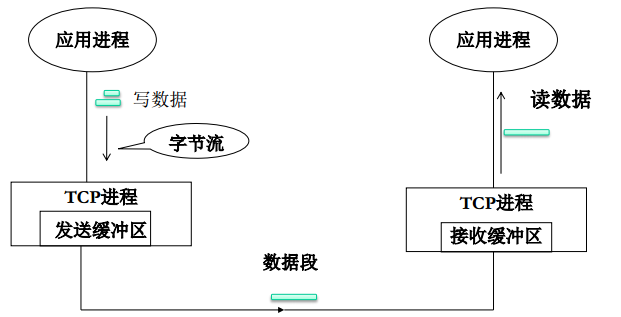
\includegraphics[width=0.5\linewidth]{fig/TCP.PNG}
\end{figure}

\begin{itemize}
\item TCP连接只能在\textemph{两个进程}间建立
\item TCP是\textemph{面向字节流}的传输方式,多次发送的数据可以放在一个数据段中传送且\textemph{不标识边界}。TCP有一个缓冲,当应用程序传送的数据块太长,TCP就可以把它划分短一些再传送。如果应用程序一次只发送一个字节,TCP也可以等待积累有足够多的字节后再构成报文段发送出去。(注意上图,是将两条写数据合并在一起变为一个数据段才发送)
\item TCP连接提供\textemph{可靠的无比特错的数据传送},但经过因特网可能出现\textemph{丢失和错序(同UDP)}。
\item 每个数据段的数据部分的\textemph{最大长度(字节)}不能超过MSS(Maximum Segment Size)\footnote{一般来讲,TCP协议会以最大传输单元(MTU)减去IP头和TCP头作为MSS。如果是以太网,则是$1500-20-20=1460$。}。
\item 客户端通过查路由表知道\textemph{IP地址},\textemph{端口号}自动选一个未用的
\end{itemize}

\subsubsection{数据段格式}
\begin{figure}[H]
    \centering
    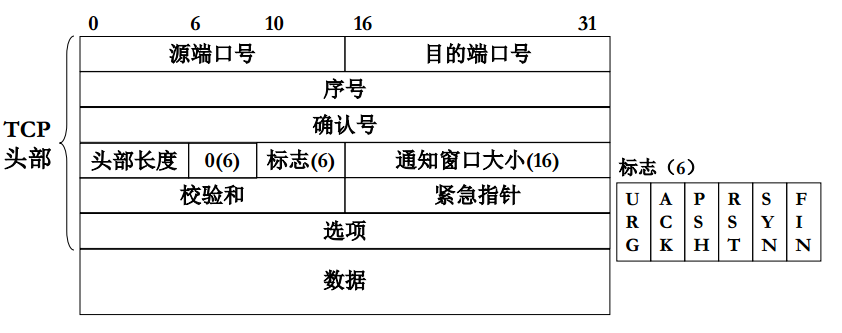
\includegraphics[width=0.8\linewidth]{fig/tcp_format.png}
\end{figure}
\begin{itemize}
    \item 序号:字节流中的\textemph{每个字节}都会被编号。
    \underline{初始序号}(initial sequence number, ISN)采用基于时间的方案, 一般采用\textemph{随机数}。
    数据部分的第一个字节的编号为\textemph{ISN+1}。
    \item 头部长度:以\textemph{字(32b)}为单位,同IP数据报。
    \item 标志:标记为1时有效
\begin{itemize}
\item SYN:同步序号标志,用来发起一个TCP连接
\item FIN:表示关闭连接,\textemph{不再发送数据},但是可以接收数据,也可以发送\textemph{数据段}(不包含数据)
\item ACK:表示确认号有效
\item PSH:告知接收方发送方执行了推送(Push)操作,接收方需要尽快将所有缓存的数据交给接收进程
\item RST:发现连接可能出了问题,连接重置
\item URG:紧急指针标志位
\end{itemize}
    \item 通知窗口(advertised window, advWin)大小:接收方告知发送方,发送方据此做出调整
    \item 校验和:由\underline{伪IP头、TCP头和TCP数据部分}形成,其形成方法与UDP协议类似。伪IP头的协议字段值为6。
    \item 紧急指针:用于指出紧急/\underline{带外数据}(out-of-band, OOB)\footnote{带外数据不属于字节流}的边界,即紧急数据的\textemph{最后一个字节的偏移量}。标志URG为1时有效。
    \begin{figure}[H]
        \centering
        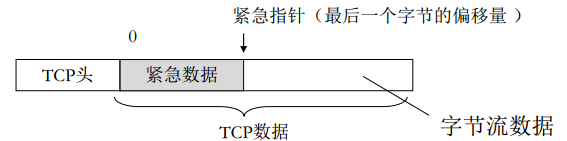
\includegraphics[width=0.5\linewidth]{fig/out-of-band.png}
    \end{figure}
    \item 选项:建立连接时有MSS、窗口比例(Scale)、是否使用选择性确认(SACK-Permitted)等。数据传送时有选择性确认的序号范围(Seletive ACK, SACK)、时间戳等。
\end{itemize}

\subsubsection{工作过程}
\begin{center}
    \begin{tikzcd}
        \text{建立连接}\arrow{r} & \text{传送数据}\arrow{r} & \text{释放连接}
    \end{tikzcd}
\end{center}
\begin{itemize}
    \item 建立连接:\textemph{非对称}活动,服务器一直在等,客户向服务器呼叫
    \item 传送数据:\textemph{全双工}方式
    \item 释放连接:\textemph{对称}活动,可由任何一方发起
\end{itemize}

\myhline
\begin{figure}[H]
    \centering
    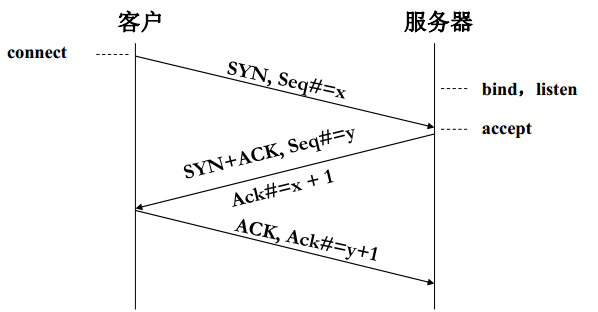
\includegraphics[width=0.6\linewidth]{fig/tcp_connect.png}
    \caption*{三次握手建立连接}
\end{figure}
\begin{itemize}
    \item 客户端需要知道服务器的IP地址和端口号。
    服务器收到客户端发来的连接请求(SYN报文)后
    \begin{enumerate}
        \item 查看是否有进程监听该端口。
        若有,则将此连接请求传给该进程;否则,服务器发RST拒绝它。
        \item 如果该进程接受连接请求,则发回SYN+ACK报文。
    \end{enumerate}
    \item 每一步均采用\textemph{超时重传},多次重发后将放弃。重发次数与间隔时间依系统不同而不同。
    \item x和y为初始序号(随机数),分别用于两个方向的数据传送。两个方向的下一个数据段的序号分别为x+1和y+1。
    \item 注意这里确认号含义与数据链路层不同,传输层的确认号是\textcolor{red}{\textemph{期待接收下一个字节}}的序号
\end{itemize}

\begin{example}
    为什么需要三次握手建立连接?
\end{example}
\begin{analysis}
    只有一次握手的话,也就是说客户端只要发送了连接请求就认为TCP已连接,也许服务器根本就不存在或者没打开。如果继续发送数据的话,浪费带宽。再说客户端也需要服务器传来的初始序号和很多选项,这个都做不到。

    如果采用两次握手,则客户端可以通过发送大量伪造的源地址连接请求,经过两次握手后服务器误以为连接已经建立,最终耗尽所有资源,使得合法的请求连接都被拒绝,无法提供正常的服务,此即DoS攻击的原理。

    即使是三次握手也无法避免DoS攻击和DDoS攻击,因为依然可以实现大量客户端同时向服务器发送连接请求,然后接收下服务器发来的确认数据包后,不再向服务器发送确认数据包(即客户端主动不进行第三次握手),那么服务器在短时间内会维护这样的半连接队列,等待队列中的客户端确认。但由于每个半连接都会耗费服务器的资源,故最终会导致资源不够用,拒绝正常的连接请求,使得正常服务无法提供。
\end{analysis}

\myhline
TCP协议传输数据采用\textemph{选择性确认}协议(\textemph{滑动窗口}),不使用NAK。只有\textemph{一个超时定时器}。
采用字节流方式,每个数据段使用其\textemph{第一个字节}的编号作为序号\footnote{数据链路层每一个帧占一个序号},按\textemph{字节}编号。

注意TCP协议中没有说明如何处理错序到达的数据段,要取决于具体实现。

\begin{figure}[H]
    \centering
    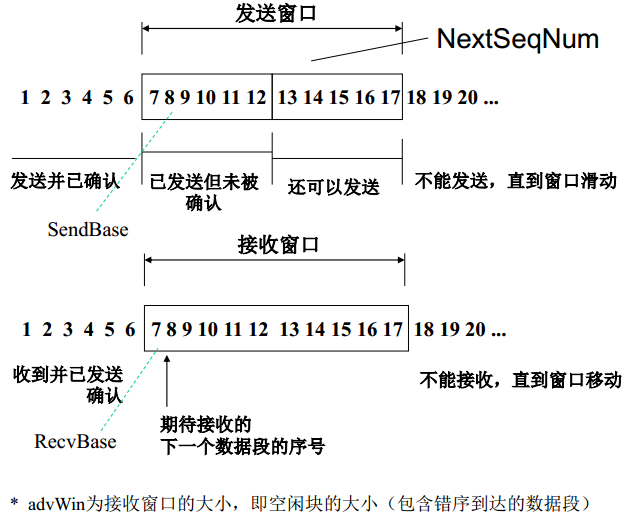
\includegraphics[width=0.6\linewidth]{fig/TCP-window.PNG}
\end{figure}
\begin{itemize}
\item 接收方先传MSS,x和接收/通知窗口大小(advWin)
\item 发送方做发送窗口,序号为x+1,大小等同advWin(接收窗口和发送窗口大小\textemph{都会改变},流控制)
\item 若接收缓冲区已满,则要等接收方进程将缓冲区取空,发送方才能继续发,否则发送窗口大小始终为0
\item 超时定时器会自动移动
\end{itemize}

\begin{example}
    下图为一个普通TCP连接的数据传送图(不使用Nagle Algorithm,Delayed ACK,Fast Retransmission,Slow start等),请填空
    \begin{figure}[H]
        \centering
        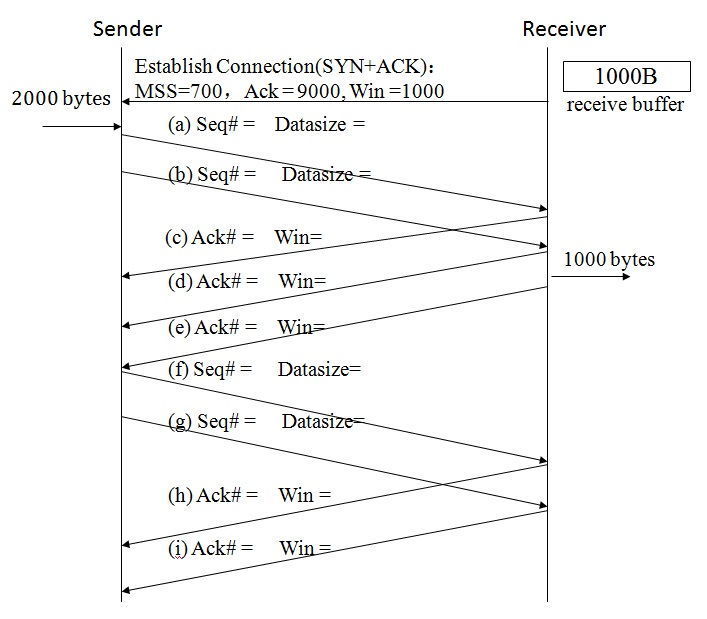
\includegraphics[width=0.5\linewidth]{fig/tcp_example.jpg}
    \end{figure}
\end{example}
\begin{analysis}
    注意窗口大小要取MSS和advWin的最小值
    \begin{enumerate}[label=(\alph*)]
        \item 9000 700,取初始序号作为Seq初值,\underline{advWin}作为\underline{sendWin初值}。发送数据段大小为\underline{MSS},因为MSS小于滑动窗口大小。
        \item 9700 300,继续将发送窗口内的字节发光,此时sendWin还是1000,只是里面的字节都已发送但未确认而已
        \item 9700 300,期待接收序号为9700,advWin减为$1000-700=300$
        \item 10000 0,期待收10000,advWin减为0,进而sendWin减为0
        \item 10000 1000,取走1000,故advWin恢复,发ACK
        \item 10000 700,重复(a)(b)(c)(d)过程
        \item 10700 300
        \item 10700 300
        \item 11000 0
    \end{enumerate}
\end{analysis}

\myhline
\begin{figure}[H]
    \centering
    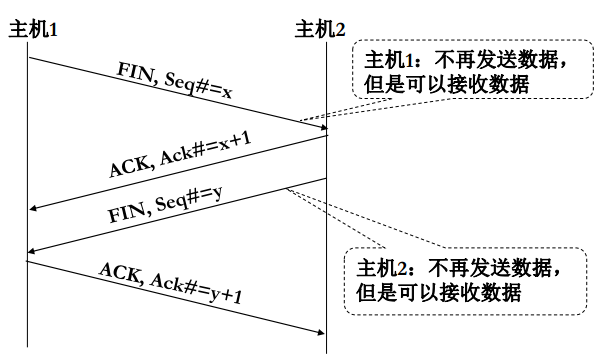
\includegraphics[width=0.6\linewidth]{fig/tcp_close.png}
    \caption*{四次握手关闭连接}
\end{figure}
\begin{itemize}
    \item FIN报文采用\textemph{超时自动重发}方式。在若干次重发后依然没有收到确认,则发送RST报文给对方后强行关闭连接。不同的系统重发方法不同。x和y都是\textemph{上一个收到的数据段的确认号}。
    \item 先发送FIN报文的一方在ACK发送完毕后需要等待\textemph{2MSL}(Maximum Segment Lifetime)的时间才\textemph{完全关闭}连接(占用端口号),用于\textemph{等待该连接的数据在因特网中消失}。TCP标准中MSL采用60秒,Unix采用30秒。
    \item 可以合并中间两次握手(ACK和FIN)或两方同时发出ACK。
\end{itemize}

\myhline
\begin{figure}[H]
    \centering
    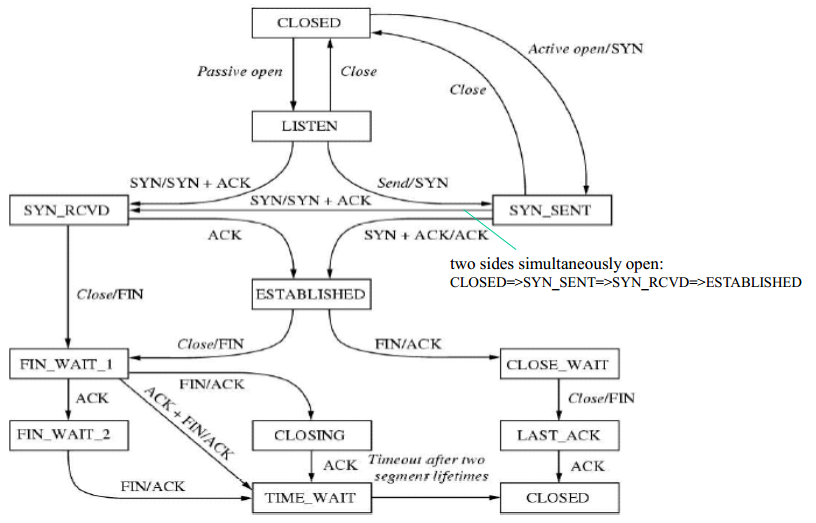
\includegraphics[width=0.8\linewidth]{fig/TCP-transition.PNG}
    \caption*{TCP协议状态转移图}
\end{figure}

\subsubsection{重传机制}
数据链路层每个帧都有一个超时定时器,而传输层只有\textemph{一个超时定时器}。
\begin{itemize}
\item \underline{快速重传}(fast retransmit):如果发送方收到一个数据段的\textemph{3次重复的ACK}(包括第一次则一共4次),它就认为其后的数据段(由确认号指出) 已经丢失,在超时之前会重传该数据段。
缺点是丢包时间很长,优点是可以减缓网络压力。
\item \underline{延迟确认}(delayed ACK):接收方并不在收到数据段立即进行确认,而是延迟一段时间再确认。如果这个期间收到多个数据段,则只需要发送一个确认。
如果在这个期间接收方有数据帧要发往发送方,还可以使用捎带确认(piggybacking)。
大部分的系统(Windows/Unix)的延迟确认时间为200毫秒。TCP标准要求延迟确认不大于500毫秒。
\item \underline{选择性确认}:接收方把收到的数据块通过数据段的选项告知发送方,使发送方不会重传这些数据块
\begin{figure}[H]
    \centering
    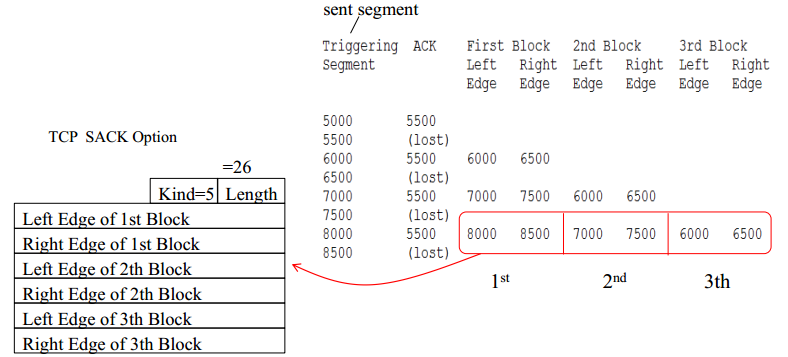
\includegraphics[width=0.8\linewidth]{fig/SACK.PNG}
\end{figure}
\end{itemize}

\subsubsection{传输层与数据链路层比较}
\begin{center}
    传输层滑动窗口协议和数据链路层的区别
\begin{tabular}{|c|c|c|}\hline
     & 传输层 & 数据链路层\\\hline
    序号 & 随机初始序号+1,按字节计数 & 每一个帧一个序号 \\\hline
确认号 & 期待接收的序号 & \begin{tabular}{l}收到哪一个就用哪一个\\代表当前与之前的全收到了\end{tabular}\\\hline
窗口大小 & 会改变 & 不会改变\\\hline
超时定时器 & \begin{tabular}{l}只有一个,只要有未确认的数据段\\就会启动(针对未确认序号最小的);\\超时没收到确认,就会重传\end{tabular} & 每个帧都有一个\\\hline
\end{tabular}
\end{center}

\subsubsection{超时计算}
数据链路层的Go back N协议由于没有中间节点,故可以用固定的超时时间(1RTT)。
而传输层涉及多个节点,故需要实时变化,进行估计。

原始公式/指数加权移动平均方法(Exponentially Weighted Moving Average, EWMA)
\[\begin{aligned}
    \text{EstimatedRTT} &= (1-\alpha)\times \text{EstimatedRTT} + \alpha \times \text{SampleRTT}\\
    \text{RTO(retransmission timeout)} &= 2\times \text{EstimatedRTT}
\end{aligned}\]
$0<\alpha<1$, $\alpha$越小过去样本的影响越大。
一般取值$\alpha=0.9$,这会使过去影响指数减少。

\myhline
TCP超时计算最常用的算法---Jacobson算法
\[\begin{aligned}
    \text{RTO} &= \text{EstimatedRTT} + 4\times \text{DevRTT}\\
    \text{DevRTT} &=(1-\beta)\times\text{DevRTT} + \beta\times|SampleRTT-EstimatedRTT|
\end{aligned}\]
在RTO计算加上一个合适的安全边际(safety margin),使得在样本变化较大时RTO会很快变得更大。
取$\alpha=1/8$,$\beta = 1/4$。
如果发送窗口为12MSS,则每12个段取样一次(采样频率)。

\myhline
Karn算法:在收到重传段确认时不要计算EstimatedRTT。
\[\text{RTO} = \gamma\times\text{RTO}\]
而是在每次重传时\textemph{直接把RTO加倍}($\gamma=2$)直到数据段首次得到确认,并把这个RTO作为后续段的RTO。
每次收到非重传段的ACK之后,就计算EstimatedRTT和正常的RTO,并用这个RTO作为后续段的RTO。
在12次重传后TCP协议发送RST并关闭连接。

\begin{example}
    如果只有最后三个连续发送的数据段被丢失,其它数据段全部收到且RTT一直保持20ms, 从这三个数据段的第一个数据段发送开始计时,还需要多少时间(ms)才可以全部收到这三个数据段的确认?
\end{example}
\begin{analysis}
    一个TCP连接的发送方只有一个超时定时器,只针对未收到确认的第一个数据段启动。\\
    采用Karn算法,第一个数据段RTO 20 + 重传时间RTT 20 = 40ms\\
    收到重传数据段确认,超时定时器移动,同时RTO加倍为40 + 重传时间RTT 20 = 60ms\\
    收到重传数据段确认,超时定时器移动,RTO加倍为80 + 重传时间RTT 20 = 100ms\\
    总数为$40+60+100=200$ms
\end{analysis}

\subsubsection{拥塞控制}
\begin{itemize}
\item 流控制:单一发送方和接收方,控制发送的速度,防止太多数据涌向\textemph{接收方}
\item 拥塞控制:防止太多数据涌向\textemph{网络},表现为\underline{丢包}(路由器上缓冲区溢出)和\underline{长延迟}(在路由器缓冲区中排队)
\end{itemize}

\myhline
拥塞控制的两大类方法:
\begin{enumerate}
    \item 端到端的拥塞控制:
\begin{itemize}
    \item 没有来自网络的明确的反馈
    \item 终端系统通过丢包和延迟推导的拥塞
    \item TCP协议的方法
\end{itemize}
    \item 网络辅助的拥塞控制:
\begin{itemize}
    \item 路由器反馈给终端系统
    \item 用一个比特指出拥塞发生(SNA, DECbit, TCP/IP ECN, ATM)
    \item 向发送方给一个明确的发送速率
\end{itemize}
\end{enumerate}
* 不主张发送ICMP包,会加重拥塞;应靠TCP自己发现拥塞。

TCP的拥塞控制属于\textemph{端到端的拥塞控制}
\begin{itemize}
    \item \underline{超时}或\underline{收到3个重复ack}就认为丢包了(同快速重传),看作拥塞发生
    \item TCP协议通过降低发送速率来控制拥塞。发送速率与发送窗口大小有关:
\[\text{发送速率(rate) $=$ SWS(Sending Window Size) $/$ RTT}\]
    \item 通过引入\textemph{拥塞窗口变量CongWin}来限制SWS。
\[SWS = \min\{\text{CongWin}, \text{AdvWin}\}\]
    CongWin为发送窗口的流量控制,AdvWin为接收方要求的流量控制
\end{itemize}

\myhline
TCP协议改变CongWin的几种机制:
\begin{itemize}
    \item 加性增乘性减(AIMD):发生拥塞\textemph{立即减半},然后\textemph{线性增长}
    \begin{figure}[H]
        \centering
        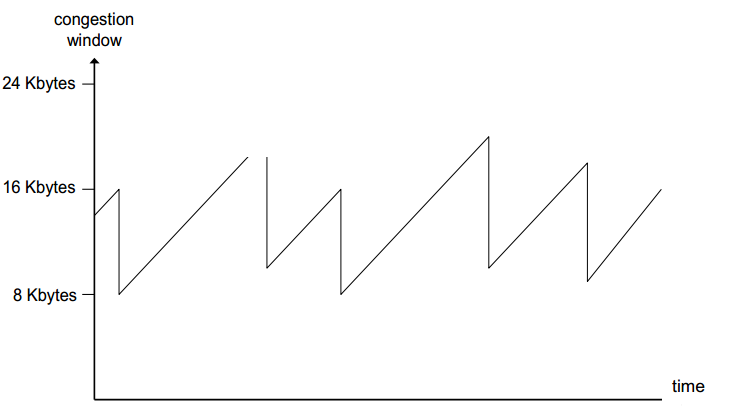
\includegraphics[width=0.5\linewidth]{fig/congression-AIMD.PNG}
    \end{figure}
    \item \underline{慢启动(slow start):Tahoe算法}
    \begin{figure}[H]
        \centering
        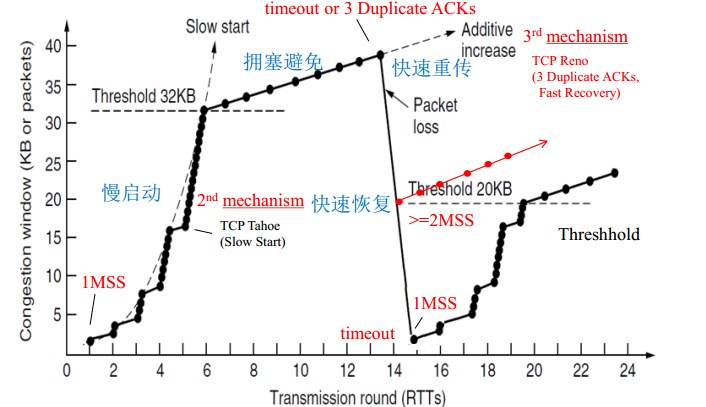
\includegraphics[width=0.8\linewidth]{fig/congression-slow-start.PNG}
    \end{figure}
    假设算法开始时通知窗口大小AdvWin=65535(用系统参数\verb'TCP_MaxWin'(一般为65535)限制CongWin的大小),SegSize为被确认的数据段的大小。
    超时或收到3个重复ACK就会触发快速重传及CongWin的变化
    \begin{enumerate}
        \item 初始时,CongWin设为1MSS, 阈值(threshold)设为65535, 发送一个数据段。
        \item 在当前窗口所有数据段的确认都收到之后, CongWin加倍。
        实际上,每收到一个确认,CongWin增加一个MSS。把它称为慢启动(slow start)是因为这个方法比立即采用advWin更慢。
        \item 当拥塞发生时,把\textemph{当前CongWin(或SWS)的一半}保存为阈值,然后CongWin又从1MSS开始慢启动(时刻0就是1MSS,上图有误)。
        \item 当CongWin增长到等于或大于阈值时,在当前窗口所有数据段的确认都收到之后, CongWin增加一个MSS(拥塞避免)。
        实际上,每收到一个ACK,CongWin增加$\text{SegSize} / \text{CongWin}$。
        如果发生拥塞,转(3)。
    \end{enumerate}
    \item \underline{快速恢复(fast recovery):Reno算法}\\
    从原来CongWin的一半开始线性增长(时刻0就是一半CongWin)
\end{itemize}

\subsubsection{存在的问题}
\textbf{问题零---关闭连接后立即又生成新的连接导致错乱}

\bigskip
\textemph{随机初始序号}和\textemph{2MSL}都用于阻止重建TCP连接相同4元组,不会收到上一次连接遗留的数据的干扰

\myhline
\textbf{问题一---长肥管道}:带宽大
\[\text{未确认的数据量capacity(b)} = \text{bandwidth(b/s)} \times \text{RTT(s)}\]
\begin{itemize}
\item \textemph{序号回绕}问题(因为速度太快):使用一般数据段的选项\verb'timestamp'(TS)。只用于区分回绕的序号是不同的,不用于确定先后次序。
也可以用Window scaling的方法,在SYN数据段选项设置WinScale(取值0-14, 默认值为0)
\[\text{sendWin} = \text{advWin} * 2^{\text{WinScale}}\]
\item \textemph{发送窗口太小},满足不了需求:当丢包发生时,由于SWS的限制,管道将会被清空。解决方法:快速重传、快速恢复。(数据链路不会,因为直连网)
\end{itemize}

\myhline
\textbf{问题二---死锁现象}:sendWin为0,接收方取空,再发不为空的ACK丢失了。
缓冲区不变化,不会发确认回来。
解决方案:
\begin{itemize}
\item 接收方可以启动一个超时定时器,可以是可以,但如果发送方没有数据传了,那接收方还是会继续发。(无谓发送数据)
\item 一般从发送方解决:在发送窗口为0之后,并且发送方有数据要发送,则启动坚持定时器(Persist Timer),定期从要发送的数据中取一个字节发送出去(Window Probe),直到收到不为0的通知窗口为止
\end{itemize}

\myhline
\textbf{问题三---傻瓜窗口症候}(silly window syndrome)
\begin{itemize}
    \item 发送进程有很多小批量数据要发送,如用telnet作为远程终端\\
    \underline{Nagle算法}---启发式算法
    \begin{figure}[H]
        \centering
        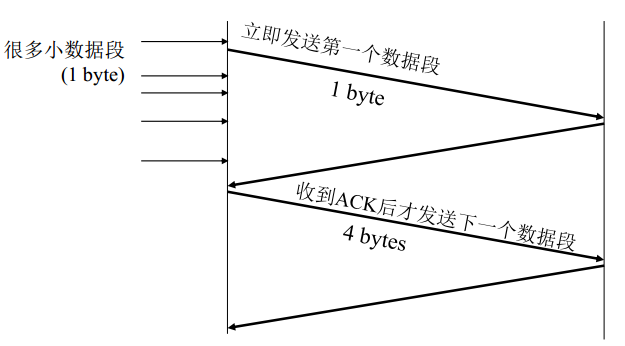
\includegraphics[width=0.6\linewidth]{fig/nagle.PNG}
    \end{figure}
    \begin{enumerate}
        \item 立即发送一个数据段,即使发送缓冲区只有一个字节
        \item 只有收到\underline{上一个数据段的确认}(此时缓冲区已经积累一定数据)或者\\\underline{发送缓冲区中数据超过MSS},才可以发送下一个数据段
        \item 对于即时性要求高的地方,如Window方式的鼠标操作,要\textemph{关闭}Nagle算法
    \end{enumerate}
    \item 接收进程频繁取走小批量数据\\
    \underline{Clark算法}:要等到接收缓冲区的空闲块大小为\underline{接收缓冲区大小的一半}\\或\underline{达到MSS}时才发送确认。
\end{itemize}

\subsubsection{定时器}
\begin{itemize}
\item 每个连接只针对第一个未确认数据段启动\underline{重传定时器}(retransmission timer)。所有数据段都已确认,则关闭它。超时重传或发送窗口移动时要重启该定时器。
\item \underline{持续定时器}(persist timer)用于保持窗口大小信息流动即使连接的另一端关闭了接收窗口。
\item \underline{保活定时器}(keepalive timer)在\textemph{长时间}没有交换数据段之后,用于检测连接的另一端是否出了问题。(如微信)隔2个小时,发10个数据段,如果没有ACK则关闭连接。(由应用层程序来做而不是TCP)
\end{itemize}